\chapter{Introduction}
\label{chp:introduction}

Over the last few years, devices capable of displaying 3D content have shown to become increasingly popular.
Most of the moviegoers have long accustomed to the variety of movies releasing in 3D every year, and with affordable 3D television screens on the market, movies with the extra dimension can be enjoyed in the living room.
It is obvious that for the viewer, the most important part of the display is the content shown by it.
Current graphics processors together with state-of-the-art rendering algorithms bring the 3D experience to the video game consumer, allowing for a higher immersion into the virtual world.
But there is also the desire to view real-world photos or videos on such a display, elevating the need for 3D capturing devices.

\section{Light Fields}

Light fields are the foundation for image based rendering, a technique to present different perspectives of a scene without the need to store geometry data, texture or lighting information.
The light field is a simplified version of the more general plenoptic function, first characterized by~\cite{AdelsonBergen}.
It can be thought of a snapshot of the light in the entire scene, a database storing the radiance for every possible ray in the scene.
This data can be captured by a grid of cameras such as the one depicted in figure~\ref{fig:stanford_camera_array}.
In fact, a light field is formed inside every conventional camera, but the per-ray radiance information is lost when the light striking the sensor is accumulated over all angles under the aperture. 
A camera that does not discard the additional radiance information is called a plenoptic camera or light field camera, shown in figure~\ref{fig:lytro_camera}.
As described by~\cite{LightFieldPhotographyHandHeldPlenopticCamera}, an application for the plenoptic camera is digital refocusing, the process of refocusing an image after it was taken.
Chapter~\ref{chp:light_field_capturing} gives an overview of the properties of light fields and how they are used in this work.

The ideal 3D display should be able to display any light field, meaning it should emit light rays with radiance equal to the value in the database.
It turns out it is not so easy to build these displays. 
On the one hand are physical challenges, such as the direction of light in different angles or the correct depiction of color, contrast and brightness.
On the other side comes a lot of data from the light field that needs to be processed, desirably in real-time and full resolution.
Despite these challenges, many types of displays have been developed, although not necessarily based around light field technology, all having different trade-offs and limitations.
There are two main categories, stereoscopic- and true 3D displays.

\begin{figure}[tb]
	\begin{subfigure}[t]{0.45\textwidth}
		\centering
		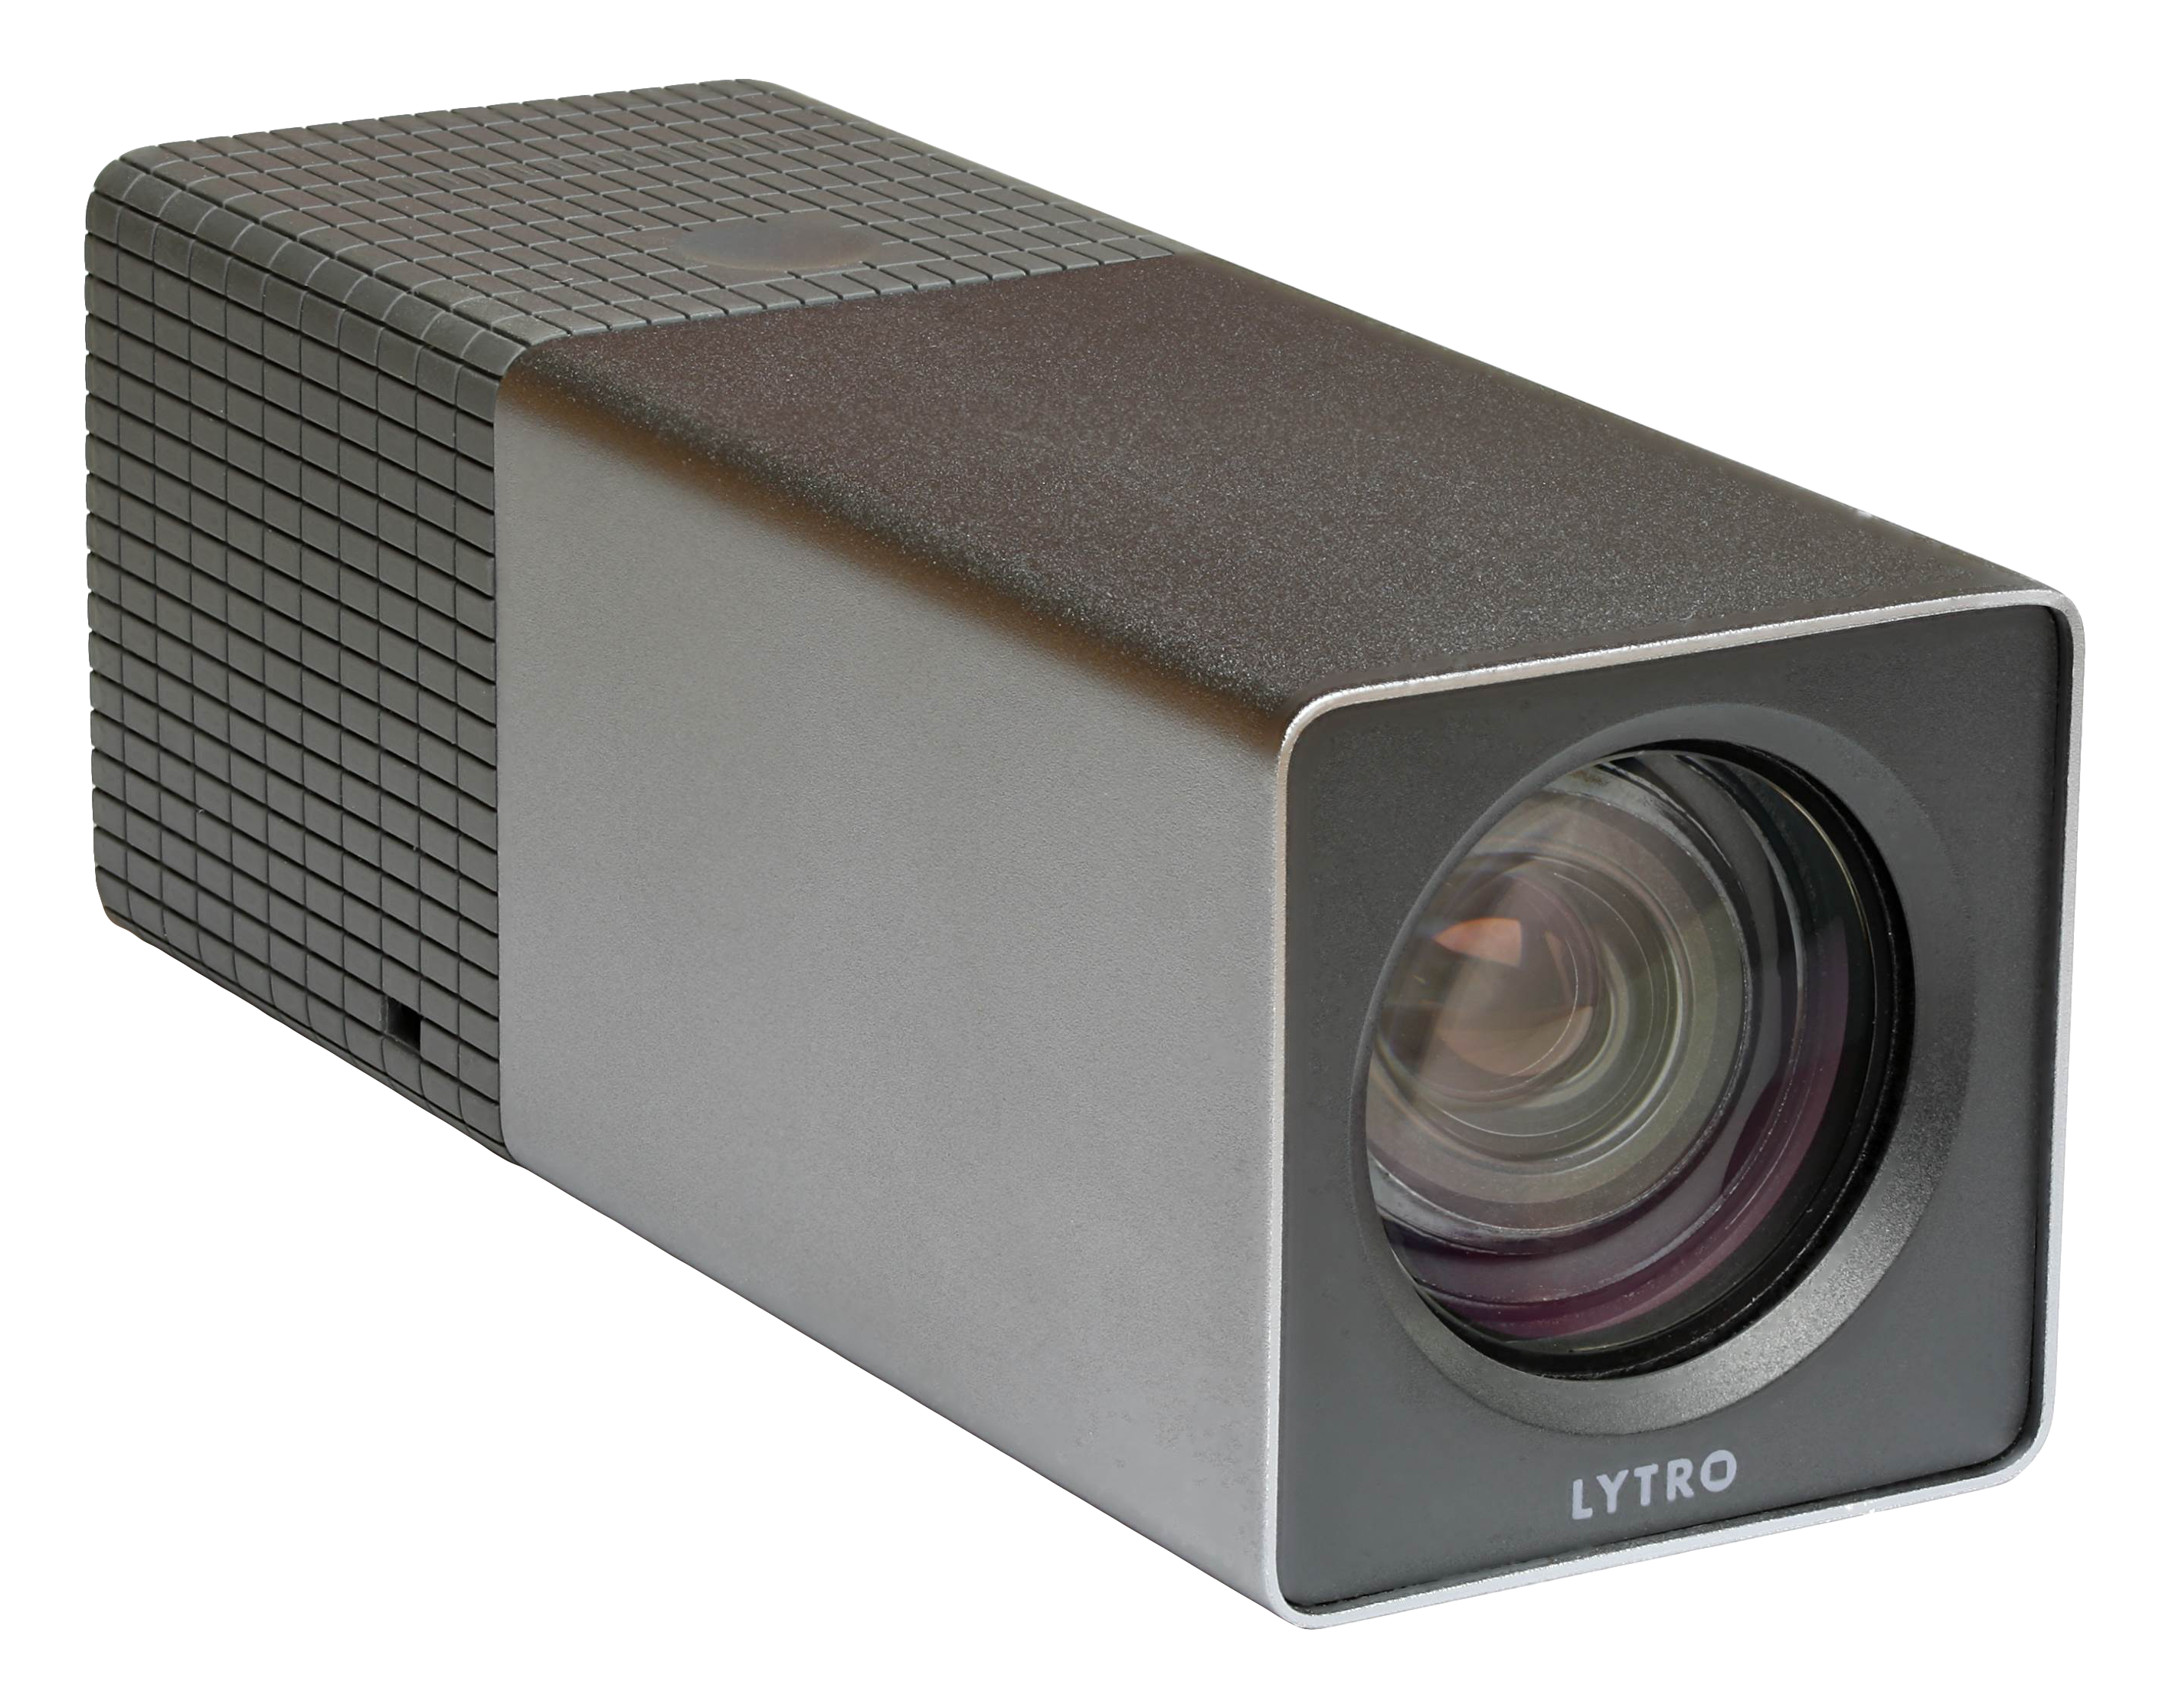
\includegraphics[height = 3.5cm]{../Figures/lytro/Lytro_Light_Field_Camera-front_background_removed}
		\caption{}
		\label{fig:lytro_camera}
	\end{subfigure}
	\hfill
	\begin{subfigure}[t]{0.45\textwidth}
		\centering
		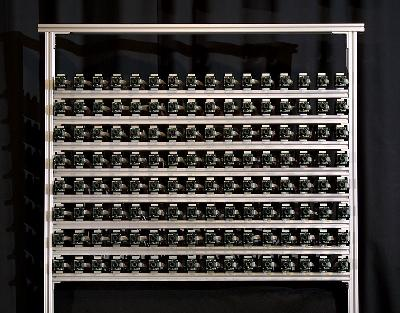
\includegraphics[height = 3.5cm]{../Figures/camera_array/stanford_camera_array_2}
		\caption{}
		\label{fig:stanford_camera_array}
	\end{subfigure}
	\caption[Light field aquisition devices]
			{(a) Hand-held plenoptic camera from Lytro. 
				 Image courtesy \mbox{D-Kuru}, \mbox{Wikimedia} Commons.
			 (b) The Stanford multi-camera array, holding 128 video cameras.
				 Image courtesy Marc Levoy, Stanford Computer Graphics Laboratory, with permission.}
\end{figure}

\section{Stereoscopic Displays}

Stereoscopic displays are based on the principles of binocular vision.
The objective is to provide two distinct images to the human visual system, one for each eye, presenting the content from two slightly different perspectives.
The disparities between the two images translate to depth cues in the human brain and allow for depth perception.
The pair of images presented to the eyes remains constant when the viewer moves in front of the device. 
This effect distinguishes stereoscopic displays from 3D displays.
Modern technologies include head-mounted displays, polarization systems, active shutter systems and autostereoscopy.
Although not as comfortable to wear, head-mounted displays have separate high resolution screens for each eye allowing for a high degree of immersion.
Polarization screens show the image pair superimposed with different polarization of the light, which is separated again by different polarization filters in the right and left side of the viewers eyeglasses.
Active shutter systems use special eyeglasses that alternately block the light for one eye, letting the opposite eye see the corresponding image on the synchronized screen.
Autostereoscopic displays present stereo content to the viewer without the need of special glasses. 
The technology is based on a lenticular lens or parallax barriers, which requires the viewer to be in a fixed and predefined position. 

\section{3D Displays}

Real 3D displays ideally show the full 3D information to the observer.
In contrast to stereoscopic displays, the person is able to move in front of the screen and view the content from a desired perspective.
Present technologies include volumetric displays, holography, integral imaging and compressive light field displays.
Volumetric displays reproduce a physical volume emitting the light of virtual objects inside, allowing for a full 360 degree viewing angle.
Holographic displays are based on conventional LCD panels equipped with a diffraction layer making it possible to project images in different directions in space.
Integral imaging devices achieve the same result with a microlens array in front of the screen similar to lenticular lenses.
Finally, compressive light field displays, also called tensor displays, consist of multiple LCD panels forming a stack of time multiplexed, light attenuating layers.

The work in this thesis is based on a much simpler version of these light field displays, called \emph{Layered 3D}, which was first realized by~\cite{WetzsteinTomo}.
The display is able to present a static, full 4D light field without the need of special glasses.
It consists of masks, printed on transparencies, which attenuate light from a backlight in a multiplicative manner.

\begin{figure}
	\centering
	\begin{subfigure}[t]{.49\textwidth}
		\centering
		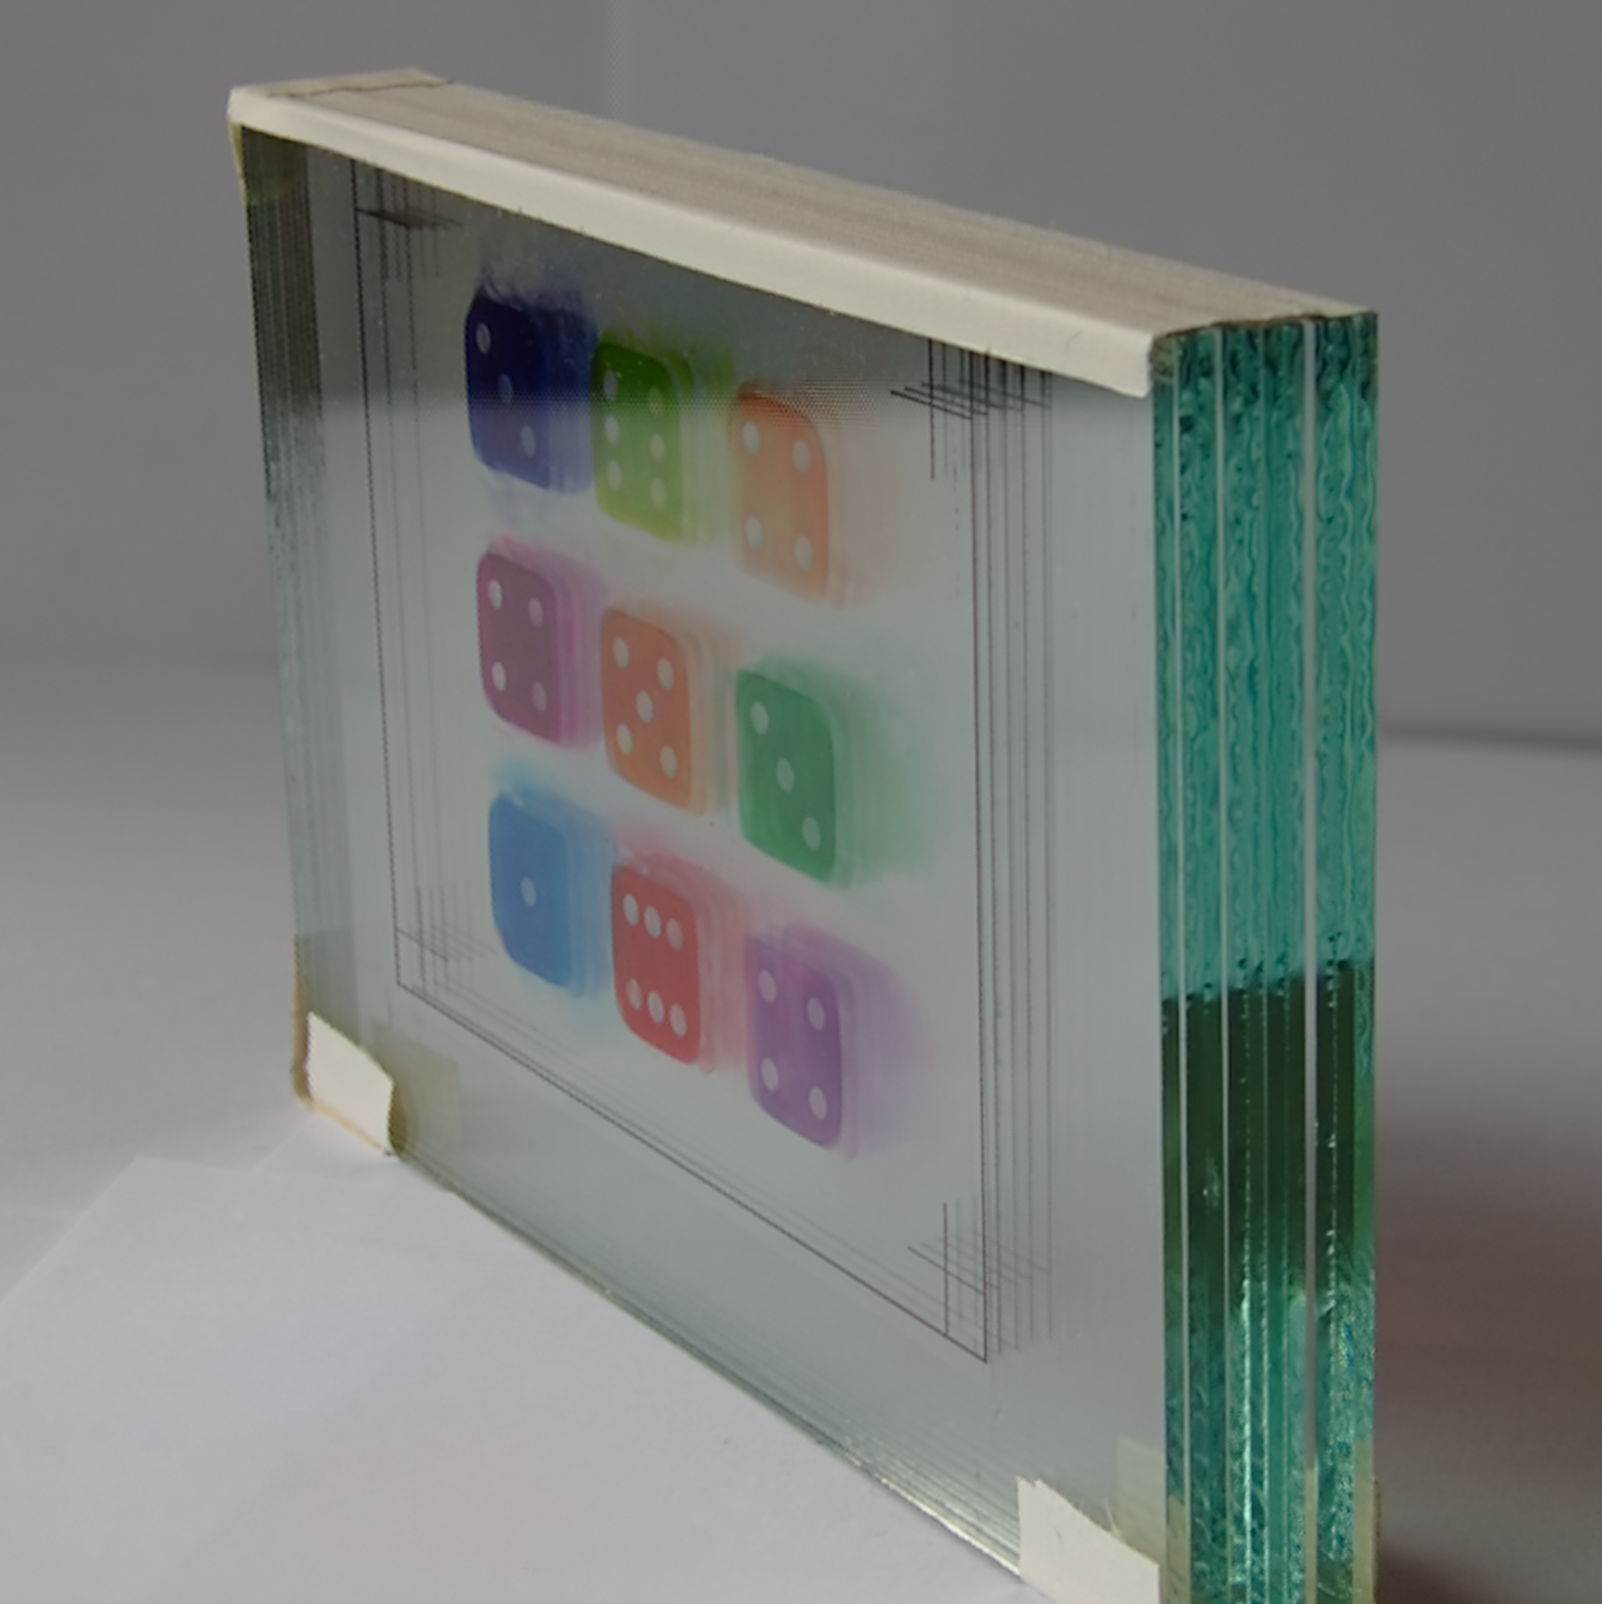
\includegraphics[width = \textwidth]{../Figures/hand_craft/glass_plates_front_view_cropped}
		\caption{}
		\label{fig:attenuation_layers_and_glasses}
	\end{subfigure}
	\hfill
	\begin{subfigure}[t]{.49\textwidth}
		 \centering
		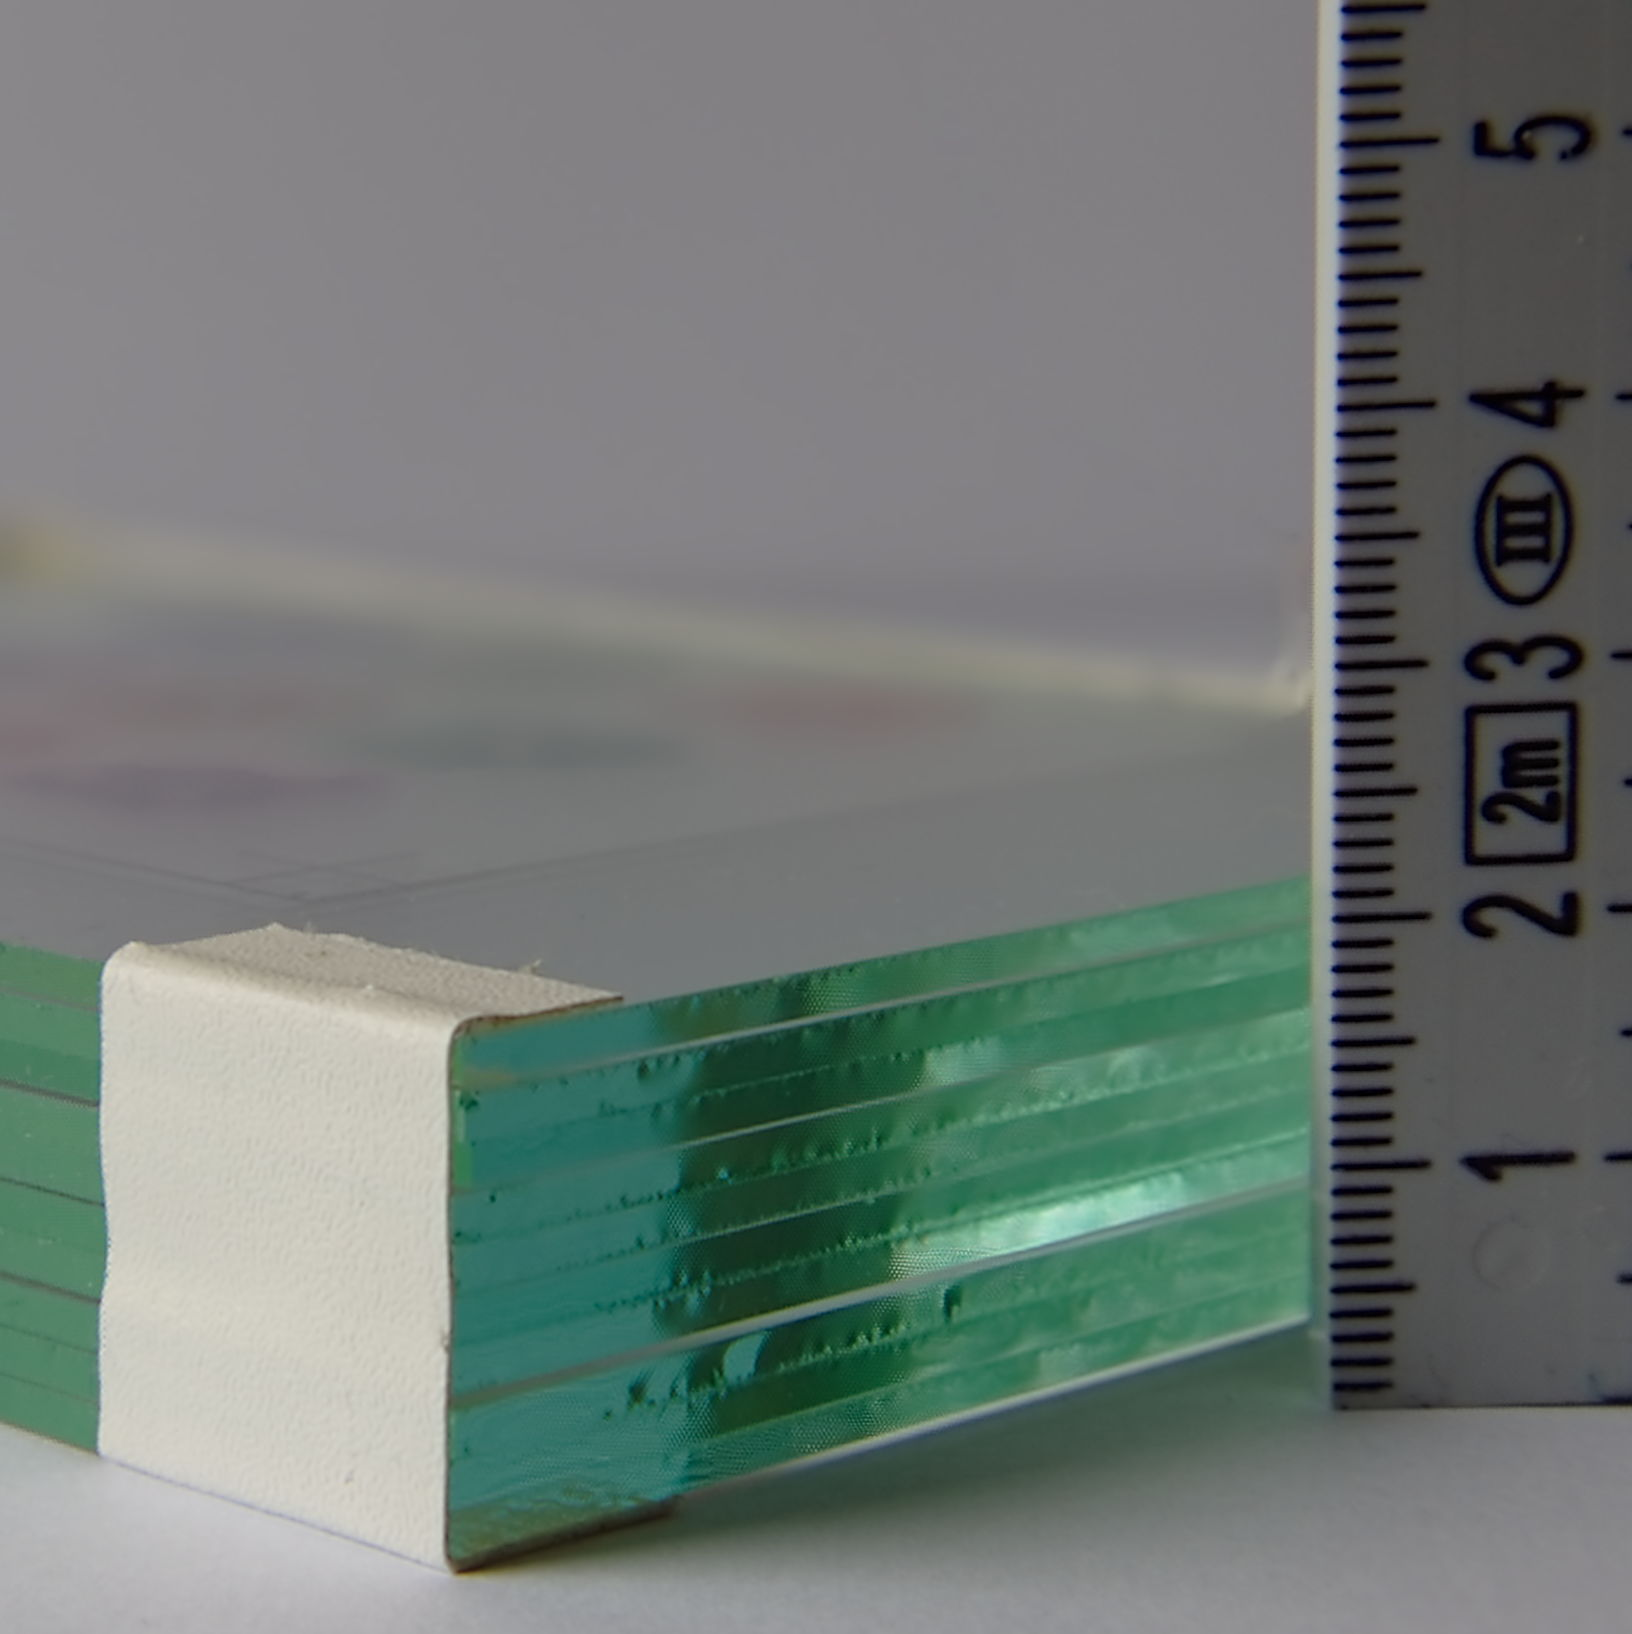
\includegraphics[width = \textwidth]{../Figures/hand_craft/glass_plates_side_view_cropped}
		\caption{}
		\label{fig:close_up_of_layers_between_glasses}
	\end{subfigure}
	\caption[Attenuation layers between glass plates]
			{Attenuation layers between glass plates.
			 (a) Front view of the display.
			 (b) Side view: Ten pieces of 2 mm thick glass plates hold the five layers of transparencies, with a 4 mm separation between them.}
	\label{fig:glass_display}
\end{figure}

\section{Related Work}

This thesis was inspired by and builds upon the work of \cite{WetzsteinTomo}.
In their paper, they present a model for an inexpensive 3D display built from light attenuating, multiplicative masks.
The simulated reconstructions they achieve are very convincing, although they only worked with synthetic light fields from oblique projections.
With a conclusive spectral analysis, they show that multi-layer displays have increased depth of field and improved spatial resolution in comparison to other automultiscopic displays such as parallax barriers or integral imaging.
The idea for this thesis was to extend their work in addition to support camera light fields, e.g. captured with a plenoptic camera or camera array.

As a followup to the original paper, \cite{WetzsteinTensor} have built a display comprising a stack of liquid crystal panels that modulate the light similar to the static layered 3D for printed transparencies.
To reduce artifacts from limited depth of field and to increase the displays field of view, they extend the degrees of freedom for the optimization by time-multiplexing a number of frames on each layer.
As a result, the observer perceives a time-average over the multi-layer frame sequence.
Their GPU-implementation solves the problem of finding the attenuation layers and frames by means of multiplicative update rules rather than tomographic reconstruction techniques, achieving interactive frame rates.

Multi-layer displays are not only suited for 3D presentation.
\cite{FocusCuesMultiPlaneDisplays} use multi-plane displays to present focus cues instead of parallax.
With their model for image formation inside the human eye, they describe the defocus effects produced in the eye when accommodating at different distances.
They compute optimal presentation layers that create a focal stack for the viewer, which handles occlusion boundaries and specularity correctly.
The proposed algorithm requires a series of images focused at different distances rather than a full 4D light field and thus requires less memory for computation.
Contrary to this work, the display planes are additive and the optimization is performed in the frequency domain.

A different application for light field displays is vision correction.
As shown by \cite{EyeglassesFreeDisplay}, light field displays can be used to pre-distort imagery in order to compensate for visual aberrations in the observers eye and to obviate the need for eyeglasses or contact lenses.
Although their physical prototype is based on parallax barriers, the concept applies for all light field displays and therefore it could also be adapted for layered 3D displays.